\chapter{Tecnología}

\section{Introducción}

El principal concepto estructural para la capa tecnológica es el nodo. Este concepto se utiliza para modelar entidades estructurales en esta capa. Es idéntico al concepto de nodo de UML 2.0. Se modela estrictamente el aspecto estructural de un sistema: su comportamiento es modelado por una relación explícita con los conceptos de comportamiento.

Una interfaz de infraestructura es la ubicación (lógica) donde los servicios de infraestructura ofrecidos por un nodo pueden ser accedidos por otros nodos o por componentes de la aplicación de la capa de aplicación.

\begin{figure}[th!]
	\centering
	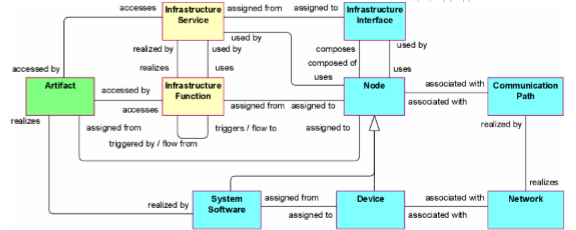
\includegraphics[width=0.7\linewidth]{arquitectura/imagenes/tecnologia}
	\caption{Metamodelo de la Capa de Tecnología}
	\label{fig:tecnologia}
\end{figure}

Las interrelaciones de los componentes de la capa tecnológica están formadas principalmente por la infraestructura de comunicación. El camino de comunicación modela la relación entre dos o más nodos, a través de los cuales estos nodos pueden intercambiar información. La realización física de un camino de comunicación es modelada con una red; es decir, un medio físico de comunicación entre dos o más dispositivos (u otras redes).


\newpage

\section{Punto de Vista de Infraestructura}

\subsection{Modelo}

\begin{figure}[th!]
	\centering
	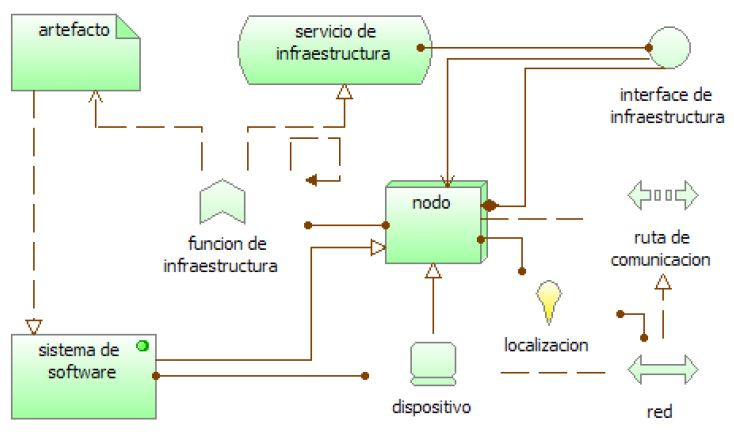
\includegraphics[width=0.7\linewidth]{arquitectura/imagenes/modeloInfraestructura}
	\caption{Metamodelo Punto de Vista Infraestructura}
	\label{metamodeloInfraestructura}
\end{figure}
El punto de vista Infraestructura contiene los elementos de infraestructura de software y hardware que soportan la capa de aplicación, como dispositivos físicos, redes o software del sistema (por ejemplo, sistemas operativos, bases de datos y middleware).

\subsection{Caso de estudio}

\begin{figure}[th!]
	\centering
	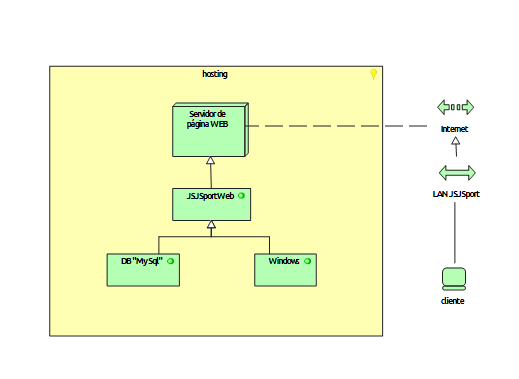
\includegraphics[width=0.6\linewidth]{arquitectura/imagenes/PuntoVistaInfraestructura}
	\caption{Modelo Punto de Vista Infraestructura}
	\label{modeloInfraestructura}
\end{figure}

Como se puede ver en la Figura 7.3 este punto de vista refleja la infraestructura necesaria para nuestra aplicación, la página WEB se ubicara en un host y dependera de un servidor WEB, además para la persistencia se hará uso de una base de datos de MySQL y ademas se hará uso de un sistema operativo Windows,el servidor WEB se comunica con internet, donde el cliente se comunica con su dispositivo a una LAN que se conecta a internet y por lo tanto a la pagina web.

\newpage

\section{Punto de Vista de Uso de Infraestructura}

\subsection{Modelo}

\begin{figure}[th!]
	\centering
	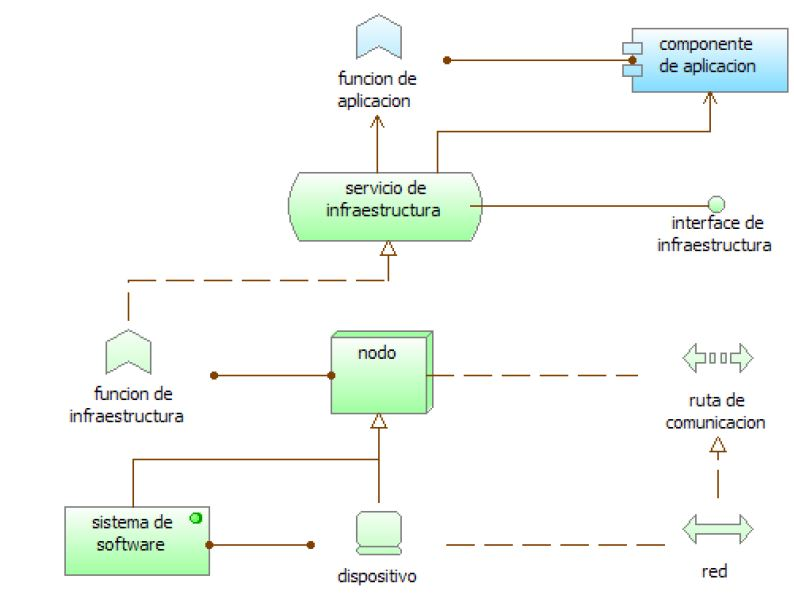
\includegraphics[width=0.6\linewidth]{arquitectura/imagenes/modeloUsoInfraestructura}
	\caption{Metamodelo Punto de Vista Uso de Infraestructura}
	\label{metamodeloUsoInfraestructura}
\end{figure}
El punto de vista de uso de la infraestructura muestra cómo las aplicaciones son compatibles con la infraestructura de software y hardware: los servicios de infraestructura son entregados por los dispositivos; Software del sistema y las redes se proporcionan a las aplicaciones. 

\subsection{Caso de estudio}

\begin{figure}[th!]
	\centering
	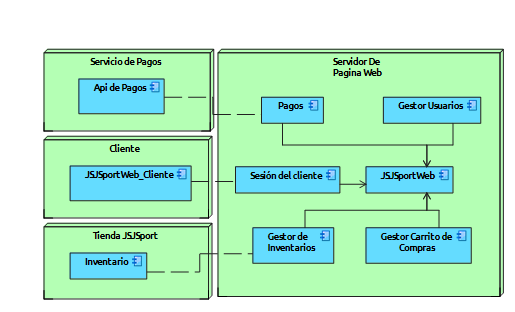
\includegraphics[width=0.6\linewidth]{arquitectura/imagenes/PuntoVistaUsoInfraestructura}
	\caption{Modelo Punto de Vista Uso de Infraestructura}
	\label{modeloUsoInfraestructura}
\end{figure}

Como se puede ver en la figura 7.5 el uso de la infraestructura esta dividido en nodos, el nodo del servidor WEB aloja todos los componentes previamente definidos de la pagina web que corresponden a la página incluyendo la principal.
\newline
Los otros 3 componentes corresponden a los nodos externos a la aplicación, el nodo del servicio de pagos provee un api que proporciona un tercer y que se encarga de los pagos este se comunica con los pagos de la aplicación y lo acopla, el nodo del cliente es lo que el cliente ve desde su ordenador y se comunica con el componente que maneja la sesión del cliente, por último se tiene el componente de inventario que se aloja en la tienda donde se maneja el inventario físico.

\newpage

\section{Punto de Vista de Implementación y Despliegue}

\subsection{Modelo}

\begin{figure}[th!]
	\centering
	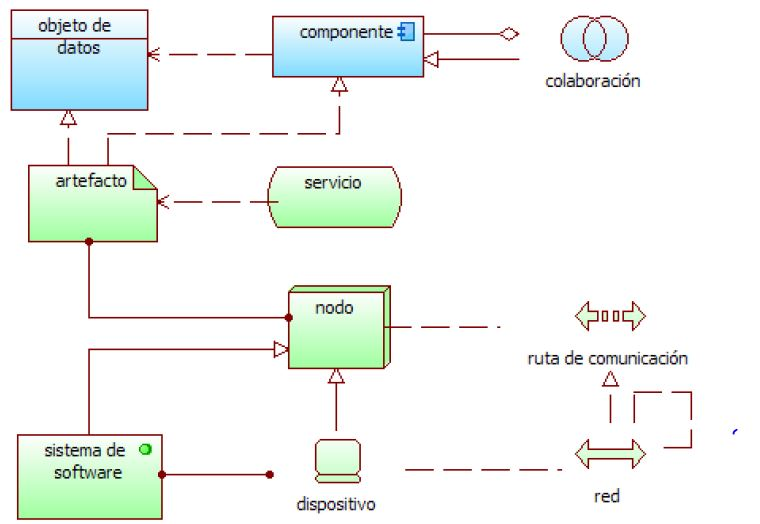
\includegraphics[width=0.5\linewidth]{arquitectura/imagenes/modeloOrganizacionImplementacion}
	\caption{Metamodelo Punto de Vista Organización e Implementación}
	\label{metamodeloOrganizacionImplementacion}
\end{figure}
El punto de vista Organización e Implementación muestra cómo se realizan una o más aplicaciones en la infraestructura. Esto comprende la asignación de aplicaciones y componentes (lógicos) o artefactos (físicos), como Enterprise Java Beans, y la asignación de la información utilizada por estas aplicaciones y componentes en la infraestructura de almacenamiento subyacente. Por ejemplo, tablas de base de datos u otros archivos. Las vistas de implementación juegan un papel importante en el análisis de rendimiento y escalabilidad, ya que relacionan la infraestructura física con el mundo lógico de las aplicaciones. En análisis de seguridad y riesgo, las vistas de implementación se utilizan para identificar, por ejemplo, dependencias y riesgos críticos.

\subsection{Caso de estudio}

\begin{figure}[th!]
	\centering
	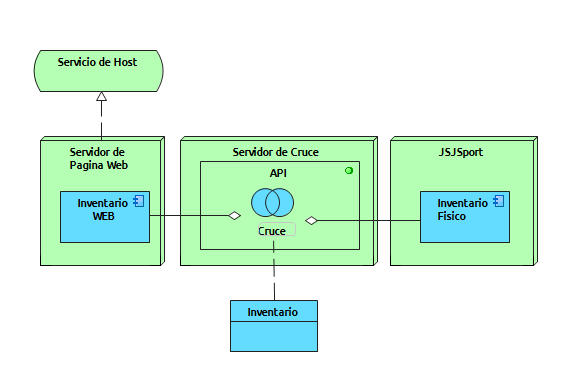
\includegraphics[width=0.7\linewidth]{arquitectura/imagenes/PuntoVistaOrganizacionImplementacion}
	\caption{Modelo Punto de Vista Organización Implementación}
	\label{modeloOrganizacion}
\end{figure}

En este punto de vista se puede observar la colaboración que existe entre el componente de inventarios de la página WEB que se aloja en el host y el componente de inventario físico que existe en la tienda de JSJSport, esta colaboración tiene luegar en un API que se encuentra en el servidor de cruce y que accede y hace uso del elemento inventario.

\newpage

\section{Punto de Vista de Estructura de la Información}

\subsection{Modelo}

\begin{figure}[th!]
	\centering
	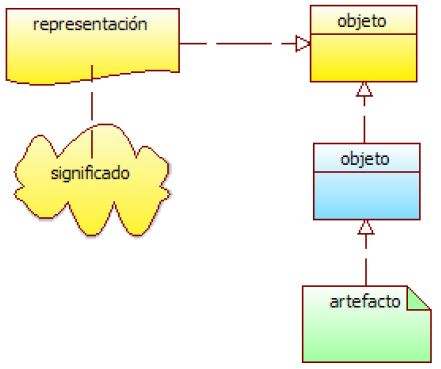
\includegraphics[width=0.5\linewidth]{arquitectura/imagenes/modeloEstructuraDeInformacion}
	\caption{Metamodelo Punto de Vista Estructura de Información}
	\label{metamodeloEstructuraInformacion}
\end{figure}
El punto de vista de la estructura de información es comparable a los modelos de información tradicionales creados en el desarrollo de casi cualquier sistema de información. Muestra la estructura de la información utilizada en la empresa o en un proceso o aplicación de negocio específico, en términos de tipos de datos o estructuras de clases (orientadas a objetos). 

\subsection{Caso de estudio}

\begin{figure}[th!]
	\centering
	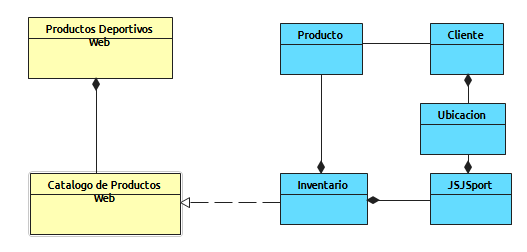
\includegraphics[width=0.7\linewidth]{arquitectura/imagenes/PuntoVistaEstructuraInformacion}
	\caption{Modelo Punto de Vista Estructura Información}
	\label{modeloEstructuraInformacion}
\end{figure}

En la figura 7.9 se puede observar como el conjunto de productos que tiene JSJSports se ve reflejado en el catalogo de productos de la empresa, del lado de la aplicación se puede ver que el inventario se ve reflejado en el catalogo de productos, este inventario tiene muchos productos y a la vez se encuentra en JSJSport que tiene una ubicación.
\newline
Al igual que JSJSport, el cliente también tiene una ubicación y no solo esto sino que también accede a los productos que tiene el inventario, todo esto desde la aplicación.


\newpage

\section{Punto de Vista de Realización del Servicio}

\subsection{Modelo}

\begin{figure}[th!]
	\centering
	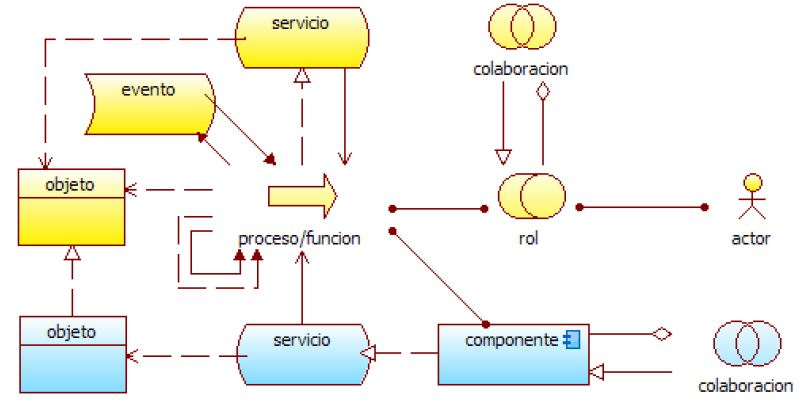
\includegraphics[width=0.7\linewidth]{arquitectura/imagenes/modeloRealizacionServicio}
	\caption{Metamodelo Punto de Vista Realización Del Servicio}
	\label{metamodeloRealizacionServicio}
\end{figure}
El punto de vista Realización del servicio se utiliza para mostrar cómo uno o más servicios empresariales son realizados por los procesos subyacentes (ya veces por los componentes de la aplicación). Por lo tanto, forma el puente entre el punto de vista de productos empresariales y la vista de procesos empresariales. 

\subsection{Caso de estudio}

\begin{figure}[th!]
	\centering
	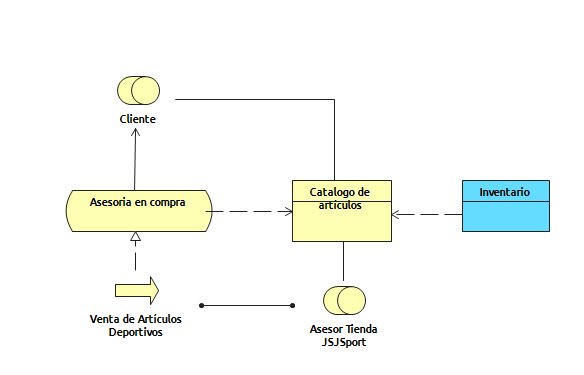
\includegraphics[width=0.7\linewidth]{arquitectura/imagenes/PuntoVistaRealizacionServicio}
	\caption{Modelo Punto de Vista Realización Servicio}
	\label{modeloRealizacionServicio}
\end{figure}

En este punto de vista se puede observar como los servicios previamente definidos en las otras capas son ejecutados por los componentes que se definieron en la capa de aplicación, en este caso el servicio de asesoría en la compra de productos deportivos esta siendo brindado a un cliente, la función de venta de artículos deportivos busca satisfacer este servicio, el encargado de realizar esta función es un asesor de la tienda, todo esto se dirige al catalogo de productos puesto que este es el tema central con el que se busca satisfacer al cliente y es la razón por la cual se comunican el cliente y el asesor, este catalogo a su vez hace uso del inventario que se encuentra en la aplicación.

\newpage

\section{Punto de Vista de Capas}

\subsection{Modelo}

\begin{figure}[th!]
	\centering
	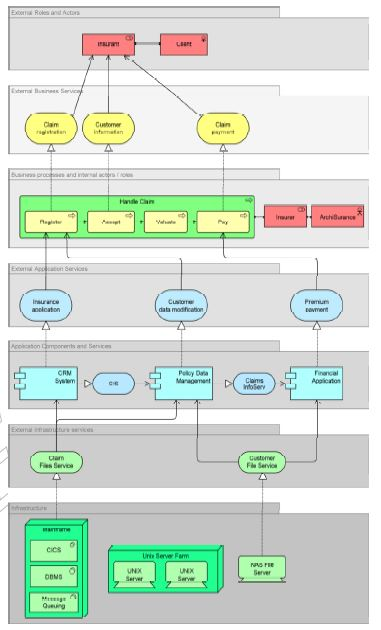
\includegraphics[width=0.6\linewidth]{arquitectura/imagenes/modeloCapas}
	\caption{Metamodelo Punto de Vista Capas}
	\label{metamodeloCapas}
\end{figure}
El punto de vista Capas muestra varias capas y aspectos de una arquitectura empresarial en un diagrama. Hay dos categorías de capas, a saber, capas dedicadas y capas de servicio. Las capas son el resultado del uso de la relación de "agrupación" para una partición natural de todo el conjunto de objetos y relaciones que pertenecen a un modelo. La infraestructura, la aplicación, el proceso y las capas de actores / roles pertenecen a la primera categoría. El principio estructural detrás de un punto de vista completamente estratificado es que cada capa dedicada expone, mediante la relación de "realización", una capa de servicios, que son "usados" por la siguiente capa dedicada.

\newpage

\subsection{Caso de estudio}

\begin{figure}[th!]
	\centering
	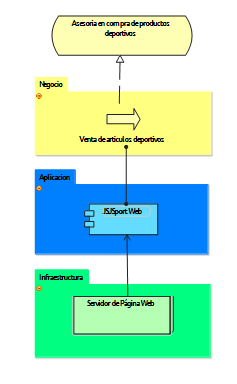
\includegraphics[width=0.7\linewidth]{arquitectura/imagenes/PuntoVistaCapas}
	\caption{Modelo Punto de Vista de Capas}
	\label{modeloCapas}
\end{figure}

Sin lugar a dudas este punto de vista que se ve reflejado en la figura 7.13 es uno de los mas importantes sino es que es el más importante puesto que refleja el trabajo hecho en las anteriores capas y como se conectan, lo principal es el servicio de la asesoría en compras de productos deportivos que se busca brindar dentro de la capa de negocio vemos la función que se realizara, dentro de la aplicación el componente que va a realizar esta función y dentro de la infraestructura podemos ver lo que nos permitirá montar concretamente la solución para lograr así satisfacer el servicio principal.

\newpage

